\documentclass[12 pt]{article}
\usepackage[utf8]{inputenc}
\usepackage{matlab-prettifier}
\usepackage[portuguese]{babel}
\usepackage{indentfirst}
\usepackage{graphicx}
\usepackage{float}
\usepackage{subcaption}
\usepackage[font=small,labelfont=bf]{caption}
\definecolor{mygreen}{RGB}{28,172,0} % color values Red, Green, Blue
\definecolor{myyellow}{rgb}{1.0, 1.0, 0.8}
\usepackage{mathtools}
\usepackage{multirow}
\usepackage{comment}
\usepackage{xcolor}
\usepackage{colortbl}
\usepackage[normalem]{ulem}               % to striketrhourhg text
\usepackage{amsmath}
\usepackage{amsfonts}
\usepackage{hyperref}
\usepackage{tcolorbox}
\usepackage{longtable}
\usepackage{enumitem}
\newcommand\redout{\bgroup\markoverwith
{\textcolor{red}{\rule[0.5ex]{2pt}{0.8pt}}}\ULon}
\renewcommand{\lstlistingname}{Código}% Listing -> Algorithm
\renewcommand{\lstlistlistingname}{Lista de \lstlistingname s}% List of Listings -> List of Algorithms

\usepackage[top=3cm,left=2cm,bottom=2cm, right=2cm]{geometry}
\usepackage{tikz}
\usetikzlibrary{decorations.pathreplacing}
\usetikzlibrary{automata}
\usetikzlibrary{positioning}
\usetikzlibrary{arrows.meta, positioning}

\usepackage{adjustbox}


% Configuração para destacar a sintaxe do Python
\lstset{ 
    language=Python,                     % A linguagem do código
    backgroundcolor=\color{myyellow}, % A cor do fundo 
    basicstyle=\ttfamily\footnotesize,   % O estilo do texto básico
    keywordstyle=\color{blue},           % Cor das palavras-chave
    stringstyle=\color{red},             % Cor das strings
    commentstyle=\color{mygreen},          % Cor dos comentários
    numbers=left,                        % Números das linhas à esquerda
    numberstyle=\tiny\color{gray},       % Estilo dos números das linhas
    stepnumber=1,                        % Número de linhas entre os números das linhas
    frame=single,                        % Moldura ao redor do código
    breaklines=true,                     % Quebra automática das linhas longas
    captionpos=t,                        % Posição da legenda
    showstringspaces=false               % Não mostra espaços em branco nas strings
    extendedchars=true,
    literate={º}{{${ }^{\underline{o}}$}}1 {á}{{\'a}}1 {à}{{\`a}}1 {ã}{{\~a}}1 {é}{{\'e}}1 {É}{{\'E}}1 {ê}{{\^e}}1 {ë}{{\"e}}1 {í}{{\'i}}1 {ç}{{\c{c}}}1 {Ç}{{\c{C}}}1 {õ}{{\~o}}1 {ó}{{\'o}}1 {ô}{{\^o}}1 {ú}{{\'u}}1 {â}{{\^a}}1 {~}{{$\sim$}}1
}


\title{%
\textbf{\huge Universidade Federal do Rio de Janeiro} \par
\textbf{\LARGE Instituto Alberto Luiz Coimbra de Pós-Graduação e Pesquisa de Engenharia} \par


\includegraphics[width=6cm]{COPPE UFRJ.png} \par

\textbf{Programa de Engenharia de Sistemas e Computação} \par

\vspace{1\baselineskip}
\textbf{\textit{Projeto de Pesquisa: Implementação de um método baseado em aprendizado por reforço para otimizar a comunicação peer-to-peer entre uma embarcação autônoma da Marinha do Brasil (VSNT-LAB) e um navio-mãe.}} \par

}

\author{\textbf{Aluno:} Luiz Henrique Souza Caldas \\ \textbf{Orientadora:} Profa. Dra. Rosa M. Leão (PESC/COPPE/UFRJ)}

\date{\today}

\begin{document}
\maketitle

\newpage

\tableofcontents

\section{Introdução}

\subsection{Contextualização}
% Apresente o USV-Lab como uma plataforma da Marinha do Brasil para pesquisa e desenvolvimento em veículos autônomos marítimos.

A navegação marítima autônoma representa avanços significativos na segurança e eficiência das atividades marítimas. Embora o conceito de navios autônomos não seja recente sua aplicação atual é ampla, com benefícios como a redução de erros humanos e a otimização de recursos. No campo militar, a navegação não tripulada tem ganhado destaque, ampliando capacidades operacionais e mitigando riscos humanos. Nesse contexto, a Marinha do Brasil, com um papel estratégico na defesa da Amazônia Azul, busca desenvolver capacidades de navegação autônoma, especialmente para missões de reconhecimento, por meio do Veículo de Superfície Não Tripulado Laboratorial (VSNT-Lab), exibido na figura~\ref{fig:intro_vsnt}. Essa iniciativa reflete a estratégia da Marinha em explorar o potencial da navegação autônoma para operações táticas avançadas\cite{douglas2024_VSNT}.

\begin{figure}[H]
    \caption{Veículo de Superfície Não Tripulado Laboratorial (VSNT-Lab)}
       \centering
       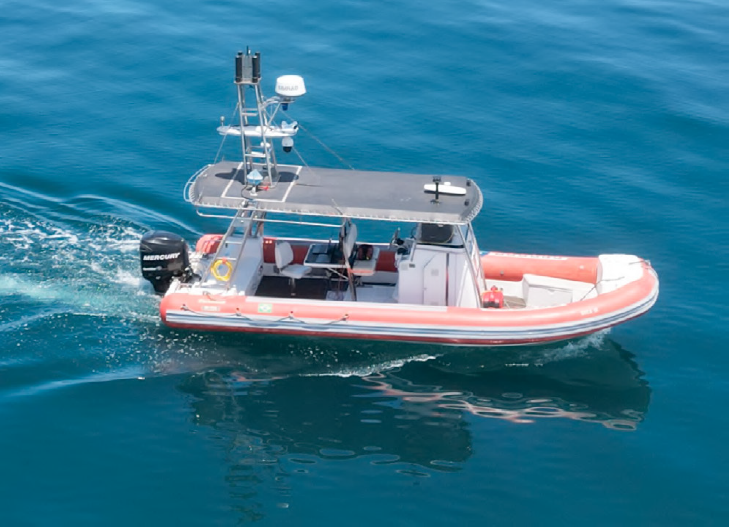
\includegraphics[height=6cm]{figuras/intro_vsnt.png}
       \label{fig:intro_vsnt}
   \small
   
   Fonte: Lima et al. \cite{douglas2024_VSNT}.
   \end{figure}


% Destaque a importância da comunicação eficiente e resiliente em missões autônomas, como as realizadas durante o exercício MINEX-23.
% Explique os desafios de manter comunicações peer-to-peer confiáveis entre o navio-mãe e o USV-Lab em cenários de operações críticas.

\subsection{Problema}
% Identifique problemas como latência, perda de pacotes e falhas de comunicação em canais mesh e VPN, que comprometem a autonomia e a eficiência das missões.

\subsection{Justificativa}
% Ressalte como a pesquisa contribui para a robustez das operações autônomas e para a segurança em missões militares e civis, alinhada aos interesses estratégicos da Marinha no "Amazônia Azul".
\section{Revisão da Bibliografia}

\subsection{Sistemas de Navegação Marítima Autônoma}
% Discuta o uso de frameworks como MOOS-IvP para controle e decisão autônoma.
% Inclua comparações entre abordagens de controle autônomo e controle humano.

\subsection{Comunicação Peer-to-Peer em Veículos Marítimos}
% Explore desafios de comunicação em redes mesh e VPNs, incluindo limitações de largura de banda e latência.

\subsection{Modelagem de QoS com HMM e RL}
% Revise estudos que aplicam Cadeias de Markov Ocultas (HMM) e Aprendizado por Reforço (RL) para prever e otimizar a qualidade de serviço em redes heterogêneas.

\subsection{Aplicações Militares de Redes Autônomas}
% Aborde o uso de Edge Computing para processamento a bordo e minimização de dependência de tráfego de dados.
\section{Objetivos}

\subsection{Objetivo Geral}
Desenvolver e implementar um método baseado em aprendizado por reforço para otimizar a comunicação peer-to-peer entre o navio-mãe e o VSNT-Lab, utilizando múltiplos canais de comunicação (rede mesh baseada em rádio NetNode e conexão VPN sobre 4G).

\subsection{Objetivos Específicos}
\begin{enumerate}
    \item Caracterizar os desafios de comunicação específicos do VSNT-Lab.
    \item Coletar dados de desempenho dos canais mesh e VPN durante missões simuladas e reais.
    \item Modelar as condições de rede com HMM, considerando diferentes cenários operacionais.
    \item Implementar um algoritmo de RL para gerenciar e otimizar a troca entre canais.
    \item Validar o método em operações no ambiente marítimo, incluindo exercícios supervisionados pela Marinha.
\end{enumerate}
\section{Metodologia}

\subsection{Descrição do Sistema}
% Apresente os componentes do USV-Lab relevantes para a comunicação, como sensores, atuadores e infraestrutura de rede (baseada em mesh e VPN via 4G).
% Explique a integração com o framework MOOS-IvP.

\subsection{Coleta de Dados}
% Descreva os experimentos para coletar métricas de QoS (latência, perda de pacotes, jitter) durante missões simuladas e reais.

\subsection{Modelagem com HMM}
% Utilize HMM para identificar estados ocultos de rede, como "rede boa", "rede degradada" e "rede indisponível".

\subsection{Implementação de RL}
% Defina o MDP (estados, ações, recompensas) para gerenciar dinamicamente a troca entre os canais mesh e VPN.

\subsection{Validação}
% Teste o método em cenários reais, como operações militares e simulações na Baía de Guanabara e na Baía de Todos os Santos.

\subsection{Ferramentas e Tecnologias}
% Detalhe as tecnologias usadas, incluindo MOOS-IvP, infraestrutura de rádio mesh e VPN, e algoritmos de RL.
\section{Conclusão}

\subsection{Resultados Esperados}
% Otimização do uso dos canais de comunicação, garantindo maior resiliência e eficiência nas missões do USV-Lab.
% Validação da aplicabilidade de HMM e RL em cenários marítimos críticos.

\subsection{Impacto do Projeto}
% Contribuir para a evolução das capacidades autônomas da Marinha do Brasil.
% Aumentar a confiabilidade e eficiência em operações de defesa e pesquisa marítima.

\subsection{Trabalhos Futuros}
% Expandir o método para incluir mais canais de comunicação, como links satelitais.
% Integrar algoritmos de fusão de sensores para melhorar a qualidade dos dados de QoS.

\bibliographystyle{abntex2-num} % Escolha o estilo de citação desejado
\bibliography{bibliografia} % Nome do arquivo .bib (sem a extensão)

\end{document}